\section{Concourse}
    Concourse je minimalistické \CI. Zjednodušeně řečeno obsahuje pouze tři základní koncepty: pipeline (projekt), job a přihlášení.

    \subsection{Architektura Concourse, možnosti konfigurace}
        Concourse využívá -- podobně jako Jenkins a GitLab -- architekturu kontrolerů (které nazývají \textit{web node}) a pracovních uzlů (\textit{worker node}). Na rozdíl od ostatních systémů ale má všechny části bezstavové. Data se persistují do externí PostgreSQL databáze. Díky tomu lze řídící rovinu libovolně škálovat a při provozu ve víc replikách má výbornou dostupnost.

        \begin{iffigure}
            \centering
            \makebox[\textwidth][c]{
                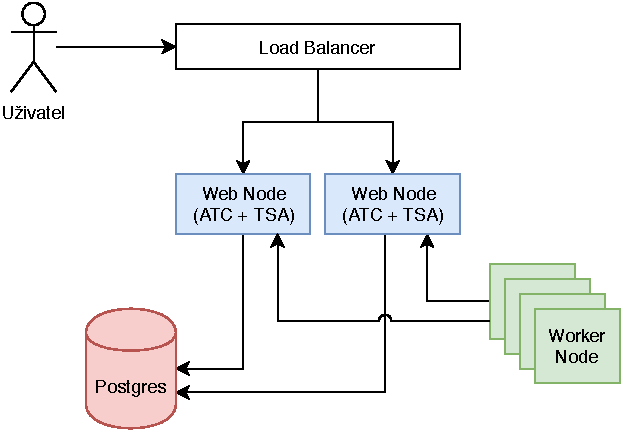
\includegraphics[width=1.0\textwidth]{media/concourse-arch.pdf}
            }
            \caption{Architektura Concourse je jednoduchá, přehledná a zároveň nabízí vysokou dostupnost. Červeně zvýrazněná PostgreSQL databáze je \glstext{SPoF}, ale díky dekompozici lze pomocí rolling update aktualizovat kontrolní rovinu bez výpadku.}
            \label{pic:concourse-architecture}
        \end{iffigure}


        \begin{figure}[H]
            \centering
                \begin{minted}[frame=lines,framesep=2mm,linenos]{ruby}
resource_types:
- name: rsync-resource
  type: docker-image
  source:
    repository: mrsixw/concourse-rsync-resource
    tag: latest

resources:
- name: repo
  type: git
  source:
    uri: "git@10.0.0.10:root/project-2.git"
    branch: master

- name: webhost
  type: rsync-resource
  source:
    server: 10.0.0.50
    base_dir: "/srv/p2"
    user: www-data
    disable_version_path: true


jobs:
- name: build
  public: true
  plan:
  - get: repo
    trigger: true
  - task: hello-world
    file: repo/concourse-task-build.yml
  - put: webhost
    params:
      sync_dir: .
                \end{minted}
                \begin{minted}[frame=lines,framesep=2mm,linenos]{ruby}
platform: linux
image_resource:
  type: docker-image
  source:
    repository: composer
    tag: 1.8
inputs:
  - name: repo
outputs:
  - name: vendor
run:
  path: composer install
\end{minted}
            \caption{Ukázka definice pipeline v Concourse. První soubor je nutné ručně nahrávat na server. Druhý soubor je definice konkrétního tasku a lze ho verzovat v aplikačním repozitáři.}
        \end{figure}

        \newpage
        Nasazení Concourse je skvěle zdokumentované a průvodní texty dokonce popisují očekávané využití procesoru a paměti pro jednotlivé komponenty. Podobně jako u~dalších distribuovaných systémů je potřeba před spuštěním jednotlivých komponent vygenerovat celou řadu klíčů. Na podepisování uživatelských session a interní komunikaci, identifikátor pro \glstext{SSH} server a pro každý \textit{worker node} jeden klíč k~registraci ke kontroleru. Další nastavení je volitelné \code{concourse-cluster}.

        Pro rychlé otestování funkčnosti a drobné projekty nabízí Concourse zjednodušenou variantu spuštění. Jedním příkazem (\code{concourse quickstart}) se spustí kontroler a worker a automaticky se pro ně vygenerují a zaregistrují potřebné klíče.

        Concourse neřeší balancování Web instancí. Je možné -- a dokonce doporučené -- mít víc než jednu repliku kontroleru, ale je na administrátorovi aby příchozí požadavky nějakým způsobem směroval, Concourse pouze na každé Web instanci vystavuje \glstext{HTTP} \code{concourse-cluster}. V~Kubernetes, OpenShift nebo podobném orchestrátoru můžeme přímo využít vestavěné služby, pro jiné systémy se ale nasazení Concourse komplikuje přidáním dalšího software pro load balancing.

        Worker instance musí být spuštěné pod root uživatelem. Podle firmy DigitalOcean je to proto, že worker potřebuje spravovat kontejnery \code{concourse-do}. To může v~základním nastavení Dockeru ale libovolný linuxový uživatel v~\code{docker} skupině~\cite{docker-postinstall}. I~s~přístupem k~Dockeru ale Concourse worker odmítal nastartovat a stále vyžadoval root uživatele.

    \subsection{Rozšiřitelnost}
        Oproti Jenkins, kde se instalují pluginy, přistupuje Concourse k~rozšiřitelnosti obráceně. Poskytuje několik základních zdrojů (pipeline, job) a \glstext{API}. Uživatelé můžou v~rámci spuštěných kontejnerů volat cokoliv potřebují. Alternativní rozhraní a podobně je možné implementovat jako externí aplikaci. Concourse se snaží dělat jednu věc a dělat jí dobře.

        Concourse lze částečně rozšířit přes koncept \textit{resources} (zdroje). Ty se balíčkují jako kontejnery a jediný požadavek na ně je, že musí obsahovat programy \code{check}, \code{in} a \code{out} v~cestě \code{/opt/resource}~\cite{concourse-resource}. Podle konfigurace konkrétní pipeline se pak periodicky volá \code{check}, který má na za úkol vrátit seznam všech nových verzí. Volání \code{in} a \code{out} má za úkol dostat nějaké informace do Concourse pipeline, resp. je nahrát z~pipeline ven. Příklad zdroje může být \glstext{RSS}, kde lze periodicky sledovat feed nějaké závislosti a při vydání nové verze automaticky spustit pipeline. Jiný příklad je zdroj git, který může nejenom reagovat na nové verze, ale i udělat nějaké změny v~repozitáři. Resource se může napojit na libovolné \glstext{API} a existují stovky opensource integrací na všechno od monitorovacích nástrojů po \CD systémy jako je Kubernetes/Helm a řada dalších~\cite{concourse-resource-list}.

        Protože některé \code{check} operace můžou být drahé a případně pomalé, přišel Concourse s~možností definovat pro zdroje také token, kterým lze programově vynutit okamžité spuštění \code{check} z~\glstext{API}. To je něco co by používala organizace pracující aktivně na několika málo z~hodně repozitářů, kde je žádoucí spustit pipeline do pár vteřin od změny, ale není praktické s~takovou periodou kontrolovat desítky repozitářů.

    \subsection{Integrace}
        Díky vysoké abstrakci v~porovnání s~ostatními \CI systémy nemusí Concourse žádné integrace řešit. To je vhodné pro správce, kteří mají míň práce. Pro hodně systémů existuje nějaká open source knihovna, která přidává integraci pomocí Concourse resource. Na rozdíl od Jenkins ale neexistuje jednotný portál, na kterém by byly všechna rozšíření zveřejněna. Na GitHubu existují stovky rozšíření, ale drtivá většina je nepoužívaná a neznámá (má malé desítky hvězd; oblíbené a často používané projekty mají stovky hvězd, například Concourse samotný jich má přes $3,5$ tisíce)~\cite{concourse-resource-list}.

        S~tím kolik práce je nějaké funkční Concourse rozšíření najít a ověřit, je často jednodušší naskriptovat integraci v~rámci pipeline. Integrace \CI do jiných systémů by měla být co nejjednodušší a Concourse se svojí obecností v~tomto ohledu strádá.

        Výhoda Concourse zdrojů oproti vlastním skriptům je dekompozice. V~rámci jedné organize je rozumné vyčlenit integrace používané ve víc projektech a pak je používat. Nejen v~tomto ohledu je Concourse nástroj vhodný pro velké korporace.
        %\todo{má to integrace na spoustu oauth (a obecně auth) viz concourse quickstart --help}\blind[1]
        %\todo{Možnosti deploy z Concourse do cílového systému; k8s, sftp, openstack, \ldots}\blind[1]

    \subsection{Zabezpečení}
        \label{subsec:concourse-security}

        Concourse má koncept týmů a přihlášení. V~rámci jednoho týmu jsou ale všichni uživatelé oprávnění k~čemukoliv. V~rámci komunity je to známý a nevyřešený problém~\cite{concourse-issue-1317}. V~roce 2018 vzniklo \glstext{RFC} které specifikuje podporu pro \glstext{RBAC}, ale implementace zatím nevznikla. Klasické řešení které se nyní používá je nasazení samostatných Concourse clusterů pro každý tým a přidělení přístupu jenom administrátorům.

        Ve veřejné databázi \glstext{CVE} nemá Concourse moc záznamů~\cite{cve-concourse}. Žádné nejsou kompletně zařazené a otagované a část z~nich nemá dopočítané ani \glstext{CVSS}. Ani při hledání v~repozitáři jsem nenašel žádné důležité nahlášené bezpečnostní problémy.

    \subsection{Dostupnost}
        Dostupnost Concourse za běžného provozu je perfektní. Díky oddělenému externímu úložišti a bezstavové kontrolní ploše lze Concourse provozovat ve vysoké dostupnosti a téměř libovolně škálovat. Ideální by bylo místo PostgreSQL používat nějakou distribuovanou \glstext{HA} databázi. V~současném návrhu je databáze \glstext{SPoF} a nelze ji jednoduše ničím nahradit.

        Díky tomu, že Concourse má veškerý stav v~Postgre, stačí zálohovat databázi. To lze dělat atomicky a často~\cite{pg-backup}.

        Concourse lze upgradovat na novější verze bez výpadku pomocí rolling update kontrolní roviny.

    \subsection{Praktické nasazení projektů}
        Navzdory skvělé dokumentaci pro nasazení Concourse clusteru bylo pro mě vytváření pipeline a jejich správa utrpení. Na rozdíl od ostatních \CI není kanonická verze pipeline v~repozitáři, ale v~Concourse. To souvisí s~tím, že concourse je hodně abstraktní a nesoustředí se jenom na stavbu aplikací. Existují zdroje~\cite{concourse-pipeline-res} které umožňují pipeline editovat, ale použití by reálně znamenalo vytvořit jednu pipeline která by byla „napevno“ nastavená v~concourse a stahovala aktuální stav repozitáře, upravila by jinou pipeline podle specifikace a následně danou pipeline spustila. Výsledek je zbytečně komplikovaný a pomalý.

        Pipeline se tak zakládají a upravují z~konzole, ne úpravou konfigurace v~repozitáři a pushnutí, takže systém nenutí vývojáře specifikaci pipeline verzovat.

        Pro mě nejvíc zmatená část Concourse je koncept \textit{task}. Tasky umožňují spustit část pipeline ze staženého resource (což může být repozitář, ale i cokoliv jiného). Lze tak drobnou část pipeline editovat jenom s~přístupem k~repozitáři, ale v~tasku nelze nastavit definici resources, jejich stažení ani jejich nahrání. Tasky mají vstup a výstup, ale jejich integrace do pipeline se řeší mimo.

        Po praktické zkušenosti s~nasazením všech tří projektů mi toto řešení přijde míň vhodné, než mít kompletní definici pipeline v~jednom souboru spravovaném přes konzoli.

        %\todo{že při vytvoření pipeline to bylo pauznuté a nešlo to z UI vyřešit a musel jsem hledat command}

        \subsubsection{Projekt 1}
            Při nasazení projektu jsem se potýkal s~náhodnými problémy, které ostatní \CI systémy neměly. Jedna z~chyb byla například kryptická zpráva \textit{volume graph is disabled}. To je známá chyba už z~roku 2016 a je o~tom, že v~dokumentaci je uveden klíč \code{image} ale Concourse očekává \code{image\_resource}~\cite{concourse-issue-402}. Banalita, ale při kombinaci se špatnou zastaralou dokumentací a malou komunitou je to zdlouhavý problém k~řešení. Další problém který jsme při implementaci měl bylo stahování Docker kontejnerů z~veřejného repozitáře. Přestože jsem nejnovější Concourse spustil na čisté \glstext{VM} přesně podle dokumentace, bylo pravděpodobně nastaveno špatně \glstext{DNS}. Po ruční editaci nameserverů jsem skončil na další těžko rozluštitelné chybě \code{unknown handle: \textit{uuid}}. Na to nepomohlo ani smazat celou pipeline a vytvořit ji znovu. Rozhodl jsem se smazat celou databázi a začít znovu. Pro testování je to bezproblémové řešení, ale Concourse mě tímto odpudil a v~produkčním prostředí mu nedůvěřuji. Ještě na další problém jsem narazil po restartu, kde se nějakým záhadným způsobem poškodil stažený Docker obraz a Concourse končil chybou, ale nestáhnul obraz znovu.

            Pro kompilaci projektu a nahrání výsledků na web server jsem využil dva zdroje. Prvního zabudovaný zdroj \code{git} sleduje repozitář projekty a při detekci změny spustí zbytek pipeline. Následně se v~jobu repozitář naklonuje a v~rámci tasku se spustí kompilace. Výsledné vystavěné soubory se pak posílají do zdroje \code{rsync-resource}, který je definovaný externím Docker obrazem. Přijatá data nahraje přes rsync na server.

            V~ukázkových definicích jsem vědomě zapsal soukromé klíče přímo v~holém čitelném textu. Concourse podporuje různé systémy pro předávání tajemství a popisuji je \pfxref{v~sekci}{subsec:concourse-security}. Nasazení těchto produktů a jejich použití bylo ale mimo rozsah této práce.

        \subsubsection{Projekt 2}
            Ukázkový projekt 2 jsem bez obtíží a rychle nasadil. Pro testy vyžadující databázi bych využil integraci s~Docker Compose~\cite{concourse-compose}, díky které lze v~jednom jobu spustit několik navzájem síťově provázaných kontejnerů.

        \subsubsection{Projekt 3}
            Pro kontejnery má Concourse speciální typ zdroje, který pro uživatele kompletně abstrahuje interní implementaci \glstext{DinD}. Na rozdíl od předchozích dvou ukázek, které v~pipeline načítaly soubor z~repozitáře definující kroky pro kompilaci, pro kontejnery toto není potřeba. Všechny verze a kroky kompilace jsou uvedeny v~\code{Dockerfile}. Na rozdíl od ostatních \CI (GitLab, Jenkins) je v~Concourse kompilace Docker kontejnerů dokonce jednodušší, než ostatní typy operací.
